% Author: Lian Zhang

\subsection{Numerical Test}
Reuters Corpus Volume I (RCV1) is an archive of over 800,000 manually categorized newswire stories recently made available by Reuters, Ltd. Topic codes were assigned to capture the major subjects of a story and  provides a good example of how controlled vocabulary schemes represent a particular perspective on a data set. The newswire stories were organized in four hierarchical parent groups: CCAT (Corporate/Industrial), ECAT (Economics), GCAT (Government/Social), and MCAT (Markets). Each of the four parent groups also includes some child groups as showed in Table \ref{RCV1}. Every story in RCV1 is classified into one child group and further belongs to the corresponding parent group. 
\begin{table}[H]\label{RCV1}
	\centering
	\begin{tabular}{|c|c|}
		\hline
		Parent Group&  The number of child groups \\
		\hline
		CCAT&   34 \\
		ECAT&   26 \\
		GCAT&   33 \\
		MCAT&   10 \\
		\hline   
		Total&  103\\
		\hline
	\end{tabular}
	\caption{The number of child groups of each parent group.}
\end{table}
\noindent Find the paper and data of RCV1 from:\\
Lewis, D. D.; Yang, Y.; Rose, T.; and Li, F. RCV1: A New Benchmark Collection for Text Categorization Research. Journal of Machine Learning Research, 5:361-397, 2004.\\ \href{https://www.csie.ntu.edu.tw/~cjlin/libsvm/}{https://www.csie.ntu.edu.tw/~cjlin/libsvm/}
\subsubsection{Binary classification}
For the purpose of binary classification, if a story belongs to the parent categories CCAT or ECAT, it is labeled by 1, otherwise it is labeled by 0. Thus, the four parent groups are classified into two classes with labels $0,1$ as follows
\begin{equation*}
	\begin{aligned}
		&\text{Label 1}: \text{CCAT(Corporate/Industrial) , ECAT (Economics)};\\ 
		&\text{Label 0}: \text{GCAT(Government/Social), MCAT (Markets)}.
	\end{aligned}
\end{equation*}
The training set has 20,242 data and 47,236 features, which means
for any data 
$$(x_i,y_i),~x_i\in \mathbf{R}^{47236},~y_i\in\{0,1\},~~~~~i=1,2,...,20242,$$
where $x_i$ is the input data and $y_i$ is the label of the input $x_i$. The test set has 677,399 data.

\subsubsection{Multi-class classification (103 classes)}
For the purpose of multi-class classification, we consider each child group as a class and every story in the same child group is assigned with the same label. RCV1 has 103 child groups so that there are 103 classes in total. The training set has 23,149 data and 47,236 features, which means
for any data 
$$(x_i,y_i),~x_i\in \mathbf{R}^{47236},~y_i\in\{0,1,...,102\},~~~~~i=1,2,...,23149,$$
where $x_i$ is the input data and $y_i$ is the label of the input $x_i$.
The test set has 781,265 data.
\subsubsection{Results of Binary classification}
We use logistic regression with the loss function (\ref{LossTwoLabels}) to perform the binary classification of RCV1. The training algorithms used are SGD, SDA, Prox-SGD and RDA
\begin{align}
\text{SGD: }W_{i+1} &= \mathop{\arg \min}_W \left\{g_i^TW + \frac{\sqrt{i}}{2}\|W-W_i\|_2^2 \right\} ,\\ 
\text{Prox-SGD: }W_{i+1}&=\mathop{\arg \min}_W \left\{ g_i^TW + \frac{\sqrt{i}}{2}\|W-W_i\|_2^2+ \lambda\|W\|_1  \right\},\\
\text{SDA: }W_{i+1} &= \mathop{\arg \min}_W \left\{ \frac{1}{i}\sum_{\tau=1}^{i} g_{\tau}^TW + \frac{1}{2\sqrt{i}} \|W\|^2_2 \right\}, \\
\text{RDA: }W_{i+1} &=\mathop{\arg\min}_W \left\{\frac{1}{i} \sum_{\tau=1}^{i}  g_{\tau}^TW+\frac{1}{2\sqrt{i}}\|W\|^2_2+\lambda\|W\|_1 \right\}, 
\end{align} 
where $g_i$ is a sub-gradient of the loss function and $\lambda$ is a parameter to control the sparsity of the solution. Figure \ref{RCV1Loss} and Figure \ref{RCV1Sparsity} shows the training loss and the weight sparsity in 50 epochs, respectively.

\begin{figure}[H]
	\centering 
	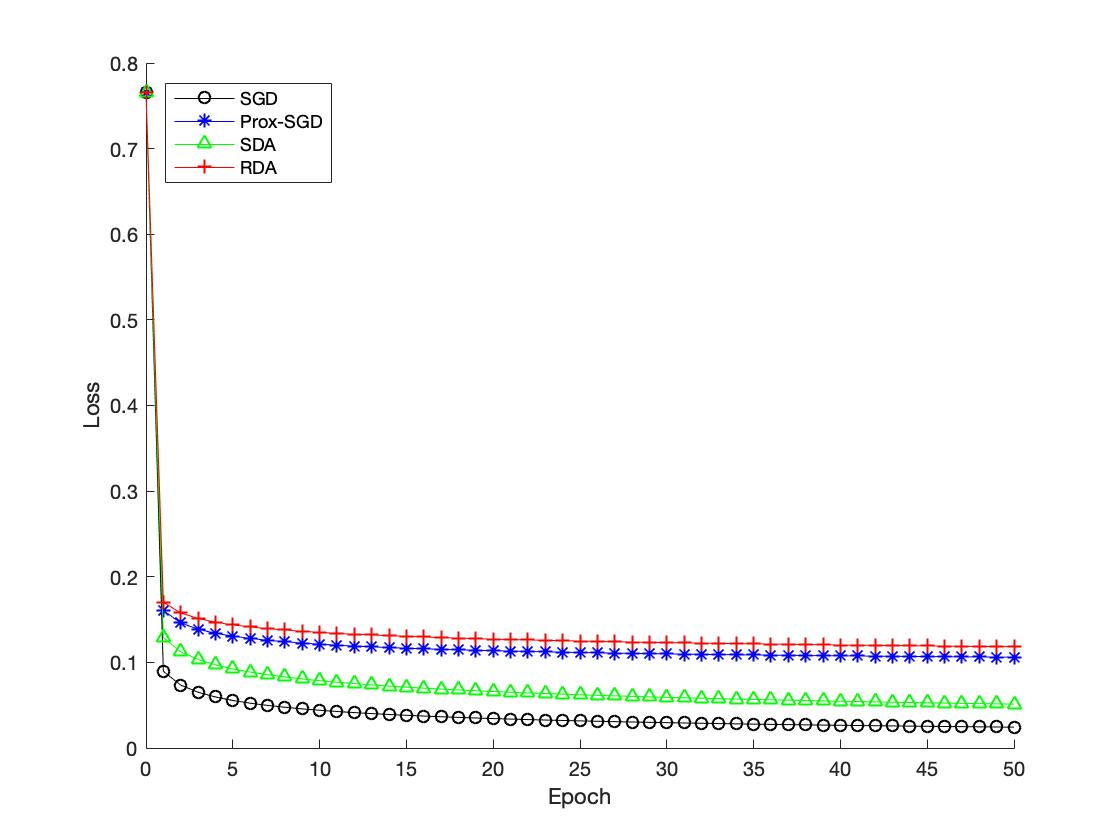
\includegraphics[scale=0.2]{./figures/LR_Loss.jpg}
	\caption{Training loss obtained by SGD, SDA, Prox-SGD and RDA in 50 epochs. For Prox-SGD and RDA, we take $\lambda=1e-5$.}
	\label{RCV1Loss}
\end{figure}
\begin{figure}[H]
	\centering 
	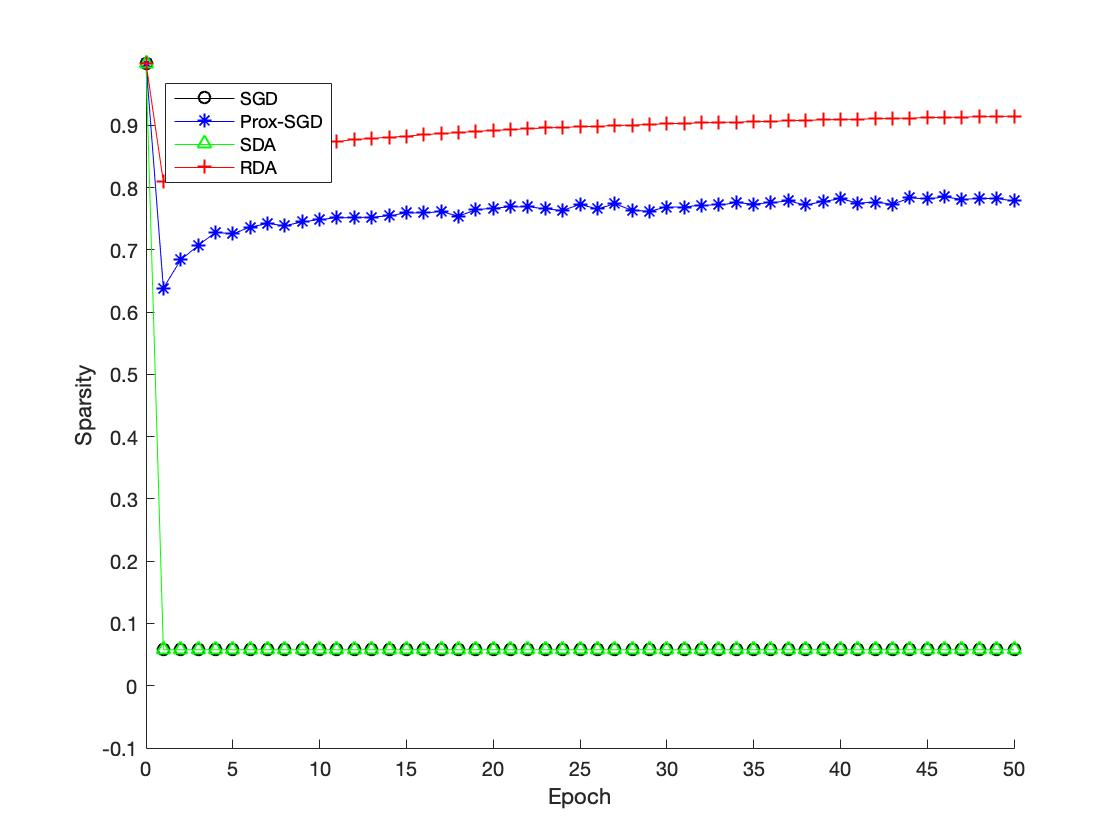
\includegraphics[scale=0.2]{./figures/LR_Sparsity.jpg}
	\caption{Weight sparsity obtained by SGD, SDA, Prox-SGD and RDA in 50 epochs. For Prox-SGD and RDA, we take $\lambda=1e-5$.}
	\label{RCV1Sparsity}
\end{figure}
